%===================================================================%
%                  VIETNAM.TEX                                      %
%===================================================================%

\documentclass{v23windows}
\hfuzz=5.002pt
\hbadness = 100000


\bibliographystyle{unsrt}    
% for BibTeX - sorted numerical labels by order of
% first citation.

% A useful Journal macro
\def\Journal#1#2#3#4{{#1} {\bf #2}, #3 (#4)}

% Some useful journal names
\def\NCA{\em Nuovo Cimento}
\def\NIM{\em Nucl. Instrum. Methods}
\def\NIMA{{\em Nucl. Instrum. Methods} A}
\def\NPB{{\em Nucl. Phys.} B}
\def\PLB{{\em Phys. Lett.}  B}
\def\PRL{\em Phys. Rev. Lett.}
\def\PRD{{\em Phys. Rev.} D}
\def\ZPC{{\em Z. Phys.} C}

% Some other macros used in the sample text
\def\st{\scriptstyle}
\def\sst{\scriptscriptstyle}
\def\mco{\multicolumn}
\def\epp{\epsilon^{\prime}}
\def\vep{\varepsilon}
\def\ra{\rightarrow}
\def\ppg{\pi^+\pi^-\gamma}
\def\vp{{\bf p}}
\def\ko{K^0}
\def\kb{\bar{K^0}}
\def\al{\alpha}
\def\ab{\bar{\alpha}}
\def\be{\begin{equation}}
\def\ee{\end{equation}}
\def\bea{\begin{eqnarray}}
\def\eea{\end{eqnarray}}
\def\CPbar{\hbox{{\rm CP}\hskip-1.80em{/}}}
\def\pt{\ensuremath{p_{\mathrm{T}}}\xspace}
\def\mjj{\ensuremath{m_{jj}}\xspace}

%\usepackage{lineno}
%\linenumbers
%temp replacement due to no font
%%%%%%%%%%%%%%%%%%%%%%%%%%%%%%%%%%%%%%%%%%%%%%%%%%
%                                                %
%    BEGINNING OF TEXT                           %
%                                                %
%%%%%%%%%%%%%%%%%%%%%%%%%%%%%%%%%%%%%%%%%%%%%%%%%%

\newcommand{\Photo}{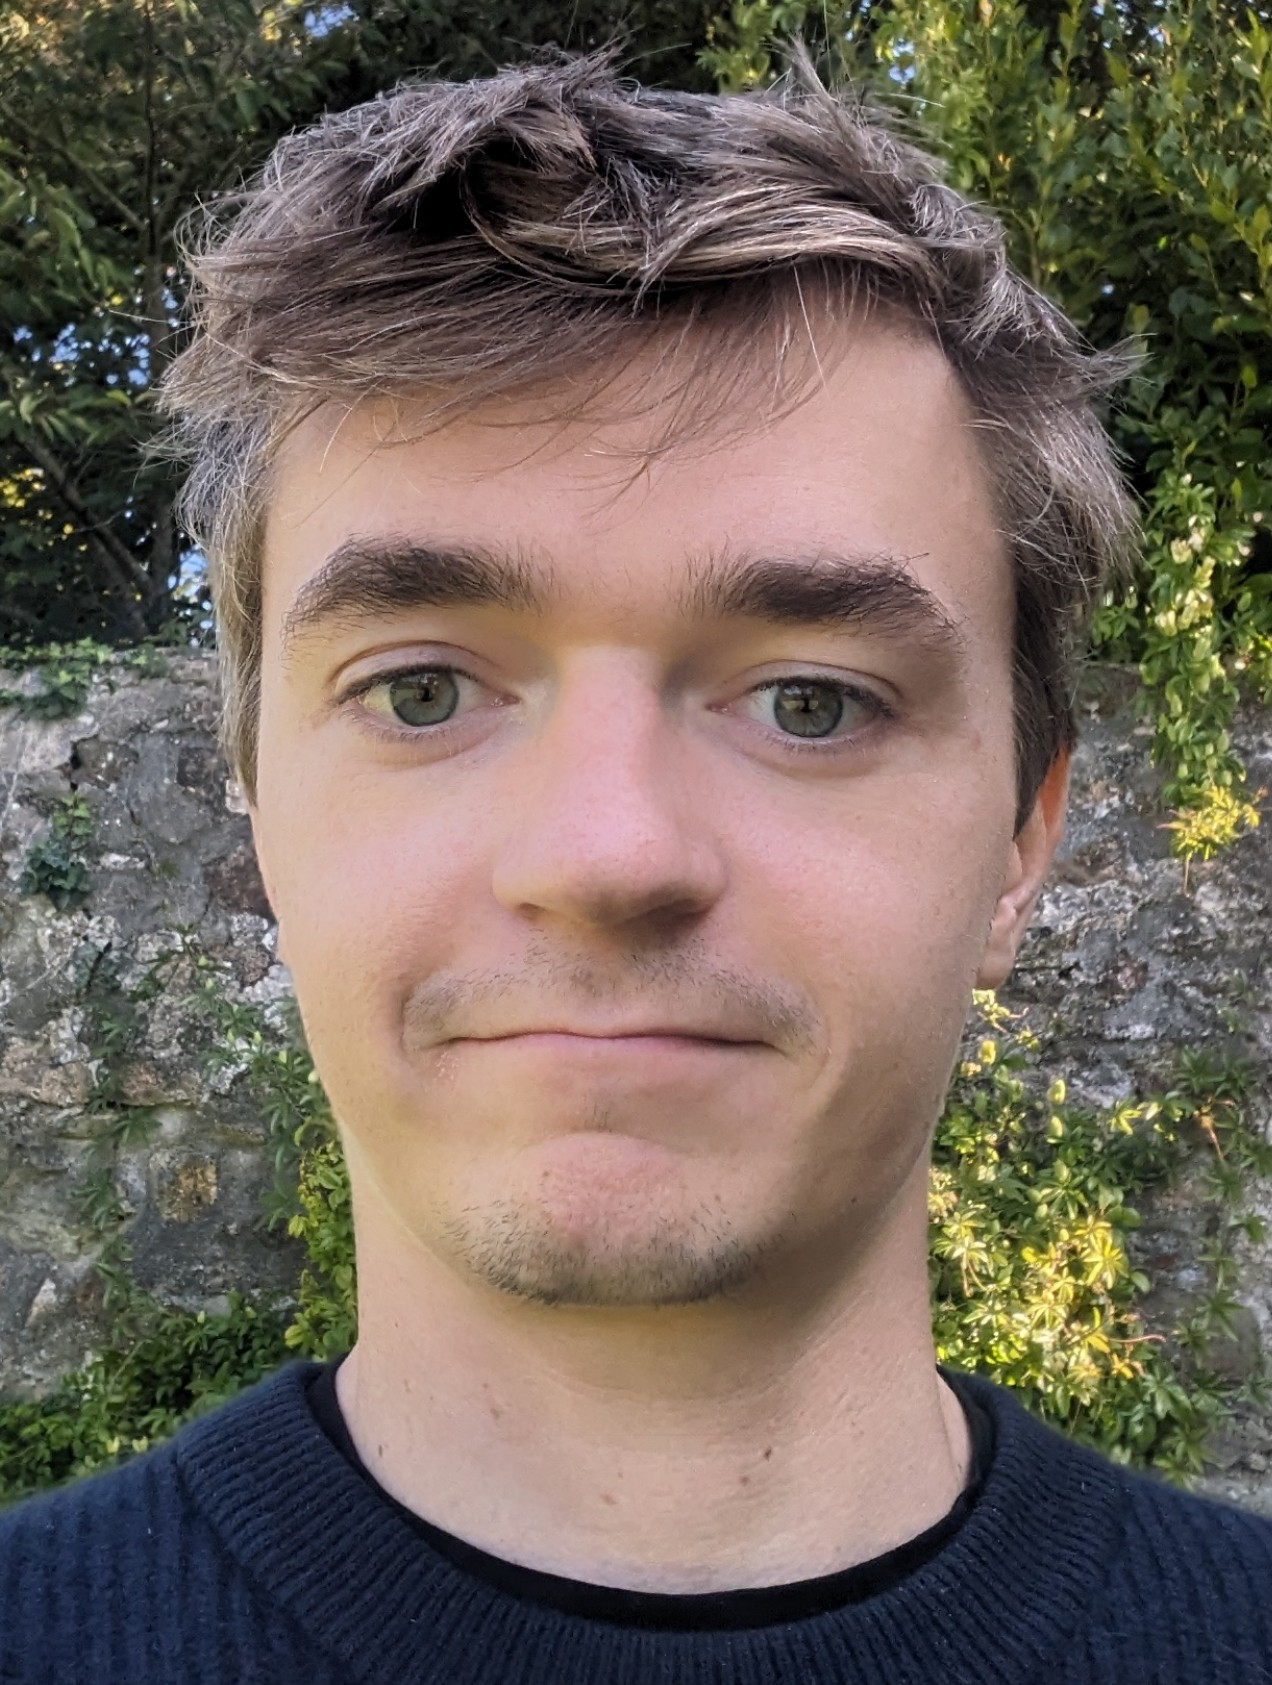
\includegraphics[height=35mm]{figures/me2.jpg}}
%\newcommand{\Photo}{}

\begin{document}
\vspace*{4cm}
\title{Studies of quartic electroweak interactions in the ATLAS experiment}

\author{ Benjamin Honan, on behalf of the ATLAS Collaboration \footnote{Copyright 2023 CERN for the benefit of the ATLAS Collaboration. CC-BY-4.0 license.} }

\address{School of Physics and Astronomy, University of Manchester, M13 9PL, United Kingdom}

\maketitle\abstracts{Processes involving quartic electroweak gauge couplings have become experimentally accessible for the first time in the run-2 dataset of the LHC. In this talk, recent measurements of triboson production and the electroweak diboson production in association with two jets by the ATLAS experiment \cite{atlas} are presented. Differential measurements of $Z\gamma\gamma$ production, as well as the observation of $W\gamma\gamma$, $WZ\gamma$ and $Z\gamma\gamma$ production are highlighted. Moreover, measurements of vector-boson scattering to $ZZ$, same-sign $WW$, and opposite-sign $WW$ are discussed. They include a large set of differential distributions in the $ZZ$, $Z\gamma\gamma$ and same-sign $WW$ channels. The results are used to constrain dimension-eight operators affecting quartic electroweak couplings in an Effective Field Theory framework.}

\section{Introduction}
%Quartic electroweak (EW) interactions appear in Vector Boson Scattering (VBS) and triboson processes at LO. These are some of rarest Standard Model processes which are still measurable at the LHC, and usually have production cross-sections of the order of femto-barnes (fb). Additionally, the strong associated production mode often forms a very large irreducible background, which can result in large modelling uncertainties on the EW measurement. This increases the difficulty associated with measuring these rare processes. The measurements of unfolded differential cross-sections of the inclusive (EW + strong + interference) and EW production can be compared to predictions from an Effective Field Theory (EFT) parametrisation, which enables the setting of limits on anomalous Quartic Gauge Couplings (aQGC). These couplings represent beyond the SM (BSM) modifications to the 4-point EW gauge boson self-interaction amplitudes. Experimentally, contributions from quartic EW interactions through VBS can be enhanced by taking advantage of the characteristic event topology consisting of two high-\pt forward jets with a large di-jet mass (\mjj) and large rapidity separation, in addition to the production of vector bosons which are produced centrally relative to these forward jets.
Quartic electroweak (EW) interactions appear in Vector Boson Scattering (VBS) and triboson processes at LO. These are some of rarest Standard Model processes which are still measurable at the LHC, and usually have production cross-sections of the order of femto-barnes (fb). The measurements of unfolded differential cross-sections of processes sensitive to EW boson self-interactions can be compared to predictions from an Effective Field Theory (EFT) parametrisation, which enables the setting of limits on anomalous Quartic Gauge Couplings (aQGC). These couplings represent beyond the SM (BSM) modifications to the 4-point EW gauge boson self-interaction amplitudes. Experimentally, contributions from quartic EW interactions through VBS can be enhanced by taking advantage of the characteristic event topology consisting of two high transverse momentum (\pt) forward jets with a large di-jet invariant mass (\mjj) and large rapidity separation ($\Delta y_{jj}$), in addition to the production of vector bosons which are produced centrally relative to these forward jets.

\section{Observation of electroweak production of $W^+W^-jj$}
$VVjj$ (where $V$ is one of $\gamma,W,Z$) processes occur via the EW and strong associated production modes (and the interference between the two modes). In the EW mode, the jets arise via the EW interaction, and in the strong mode, the jets arise via the strong interaction. An observation and fiducial cross-section measurement of the EW production of opposite-sign WW in association with jets (EW $W^+W^-jj$) is made using the ATLAS detector \cite{osww}. EW $W^+W^-jj$ is sensitive to quartic EW interactions through VBS. The signal region is defined by requiring events to pass: 2-3 jets; an opposite sign electron-muon pair; missing transverse energy $E_\mathrm{T}^{\mathrm{miss}}$ $>$ 15 GeV; and a b-jet veto.
%\begin{itemize}
%       \item 2-3 jets
%       \item An opposite sign electron-muon pair
%       \item $E_\mathrm{T}^{\mathrm{miss}}$ $>$ 15 GeV
%       \item b-jet veto
%\end{itemize}
In addition, there are requirements on the third lepton, the dilepton centrality and invariant mass, and lepton isolation and ID.  
A neural network (NN) is trained to distinguish the EW signal from the dominant backgrounds which are the strong production mode of opposite-sign WW, and backgrounds involving top decays. To constrain the dominant background from tops, a top-enriched control region is defined by inverting the b-jet veto requirement. \\\\
The significance of the observation is determined through a profile-likelihood fit with NN score in the signal and control regions simultaneously. The signal strength, and the strong and top background normalisations are included as floating parameters in the fit. By evaluating the likelihood-ratio test statistic for the background-only hypothesis, EW $W^+W^-jj$ is observed at a significance of $7.1\sigma$. A cross-section of $2.65^{+0.52}_{-0.48}$fb is measured for EW $W^+W^-jj$ in a signal-enriched fiducial volume. The dominant sources of uncertainty are statistical in nature. 

\section{Measurement of electroweak production of $W^\pm W^\pm jj$\label{sec:ssww}}
Integrated and differential fiducial cross-section measurements of the EW production of same-sign WW in association with jets (EW $W^\pm W^\pm jj$) is made using the ATLAS detector. The differential measurements are used to constrain aQGCs, and to put limits on the doubly-charged Higgs ($H^{\pm\pm}$) within the Georgi-Machacek (GM) model. \cite{ssww}
EW $W^\pm W^\pm jj$ is sensitive to VBS, quartic EW interactions, and the production of $H^{\pm\pm}$ through same-sign WW vector boson fusion (VBF). A signal region is defined by selecting for 2 same-sign leptons + third lepton veto, $E_\mathrm{T}^{\mathrm{miss}}$ $>$ 30 GeV, dilepton invariant mass $m_{ll}>$ 20 GeV, a VBS event topology, 
%\begin{itemize}
%       \item 2 same-sign leptons + third lepton veto
%       \item $E_\mathrm{T}^{\mathrm{miss}}$ $>$ 30 GeV, dilepton invariant mass $m_{ll}>$ 20 GeV
%       \item VBS event topology
%\end{itemize}
in addition to lepton \pt requirements, a Z-veto in the $ee$ channel, and requiring at least two jets. The dominant background for EW $W^\pm W^\pm jj$ is the strong associated production of $WZjj$, and notably is not the $W^\pm W^\pm jj$ strong production mode because this is uniquely suppressed in the same-sign channel. Fiducial integrated cross-sections of $\sigma_{\mathrm{EW}}=2.88\pm0.22(\mathrm{stat}.)\pm0.19(\mathrm{syst.})$ fb, and $\sigma_{\mathrm{EW+Int+QCD}}=3.35\pm0.22(\mathrm{stat}.)\pm0.20(\mathrm{syst.})$ fb are measured for the EW and inclusive (referring to the combined EW and strong production, in addition to the interference) production respectively. Differential cross-section measurements for the EW and inclusive production of $W^\pm W^\pm jj$ are derived for $m_{ll}$, $m_{\mathrm{T}}$, $m_{jj}$, $N_{\mathrm{gapjets}}$, and $\xi_{j3}$. These represent the dilepton invariant mass, $WW$ transverse mass reconstructed using $E_\mathrm{T}^{\mathrm{miss}}$ and leptons, dijet invariant mass, the number of jets in the forward jet rapidity gap, and the Zeppenfeld variable of the third jet. 
The unfolding, differential signal extraction, and $WZ$ background normalisation is performed simultaneously in a binned log-likelihood fit.\\\\
\begin{figure}
       \begin{minipage}{6in}
           \centering
           \raisebox{-0.5\height}{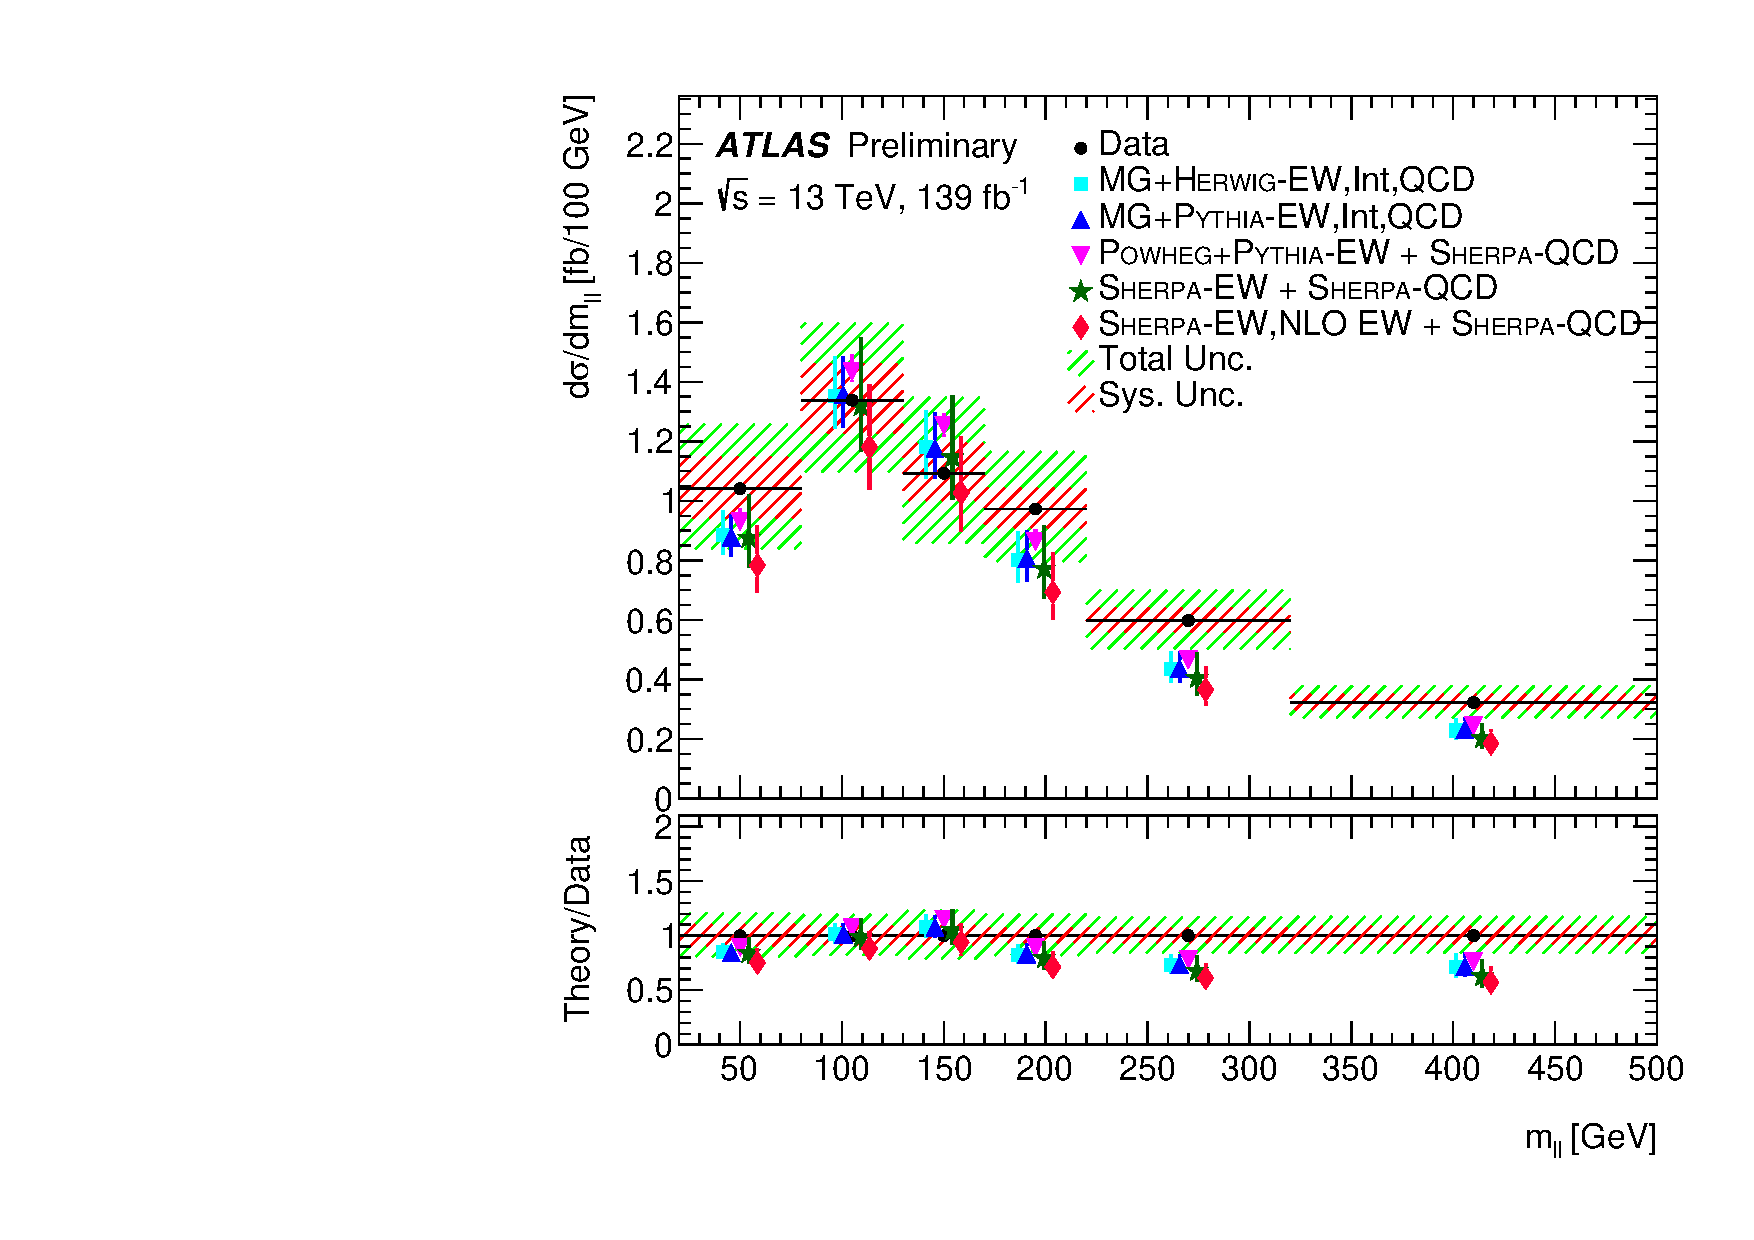
\includegraphics[width=0.49\textwidth]{figures/fig_06a.pdf}}
           \raisebox{-0.5\height}{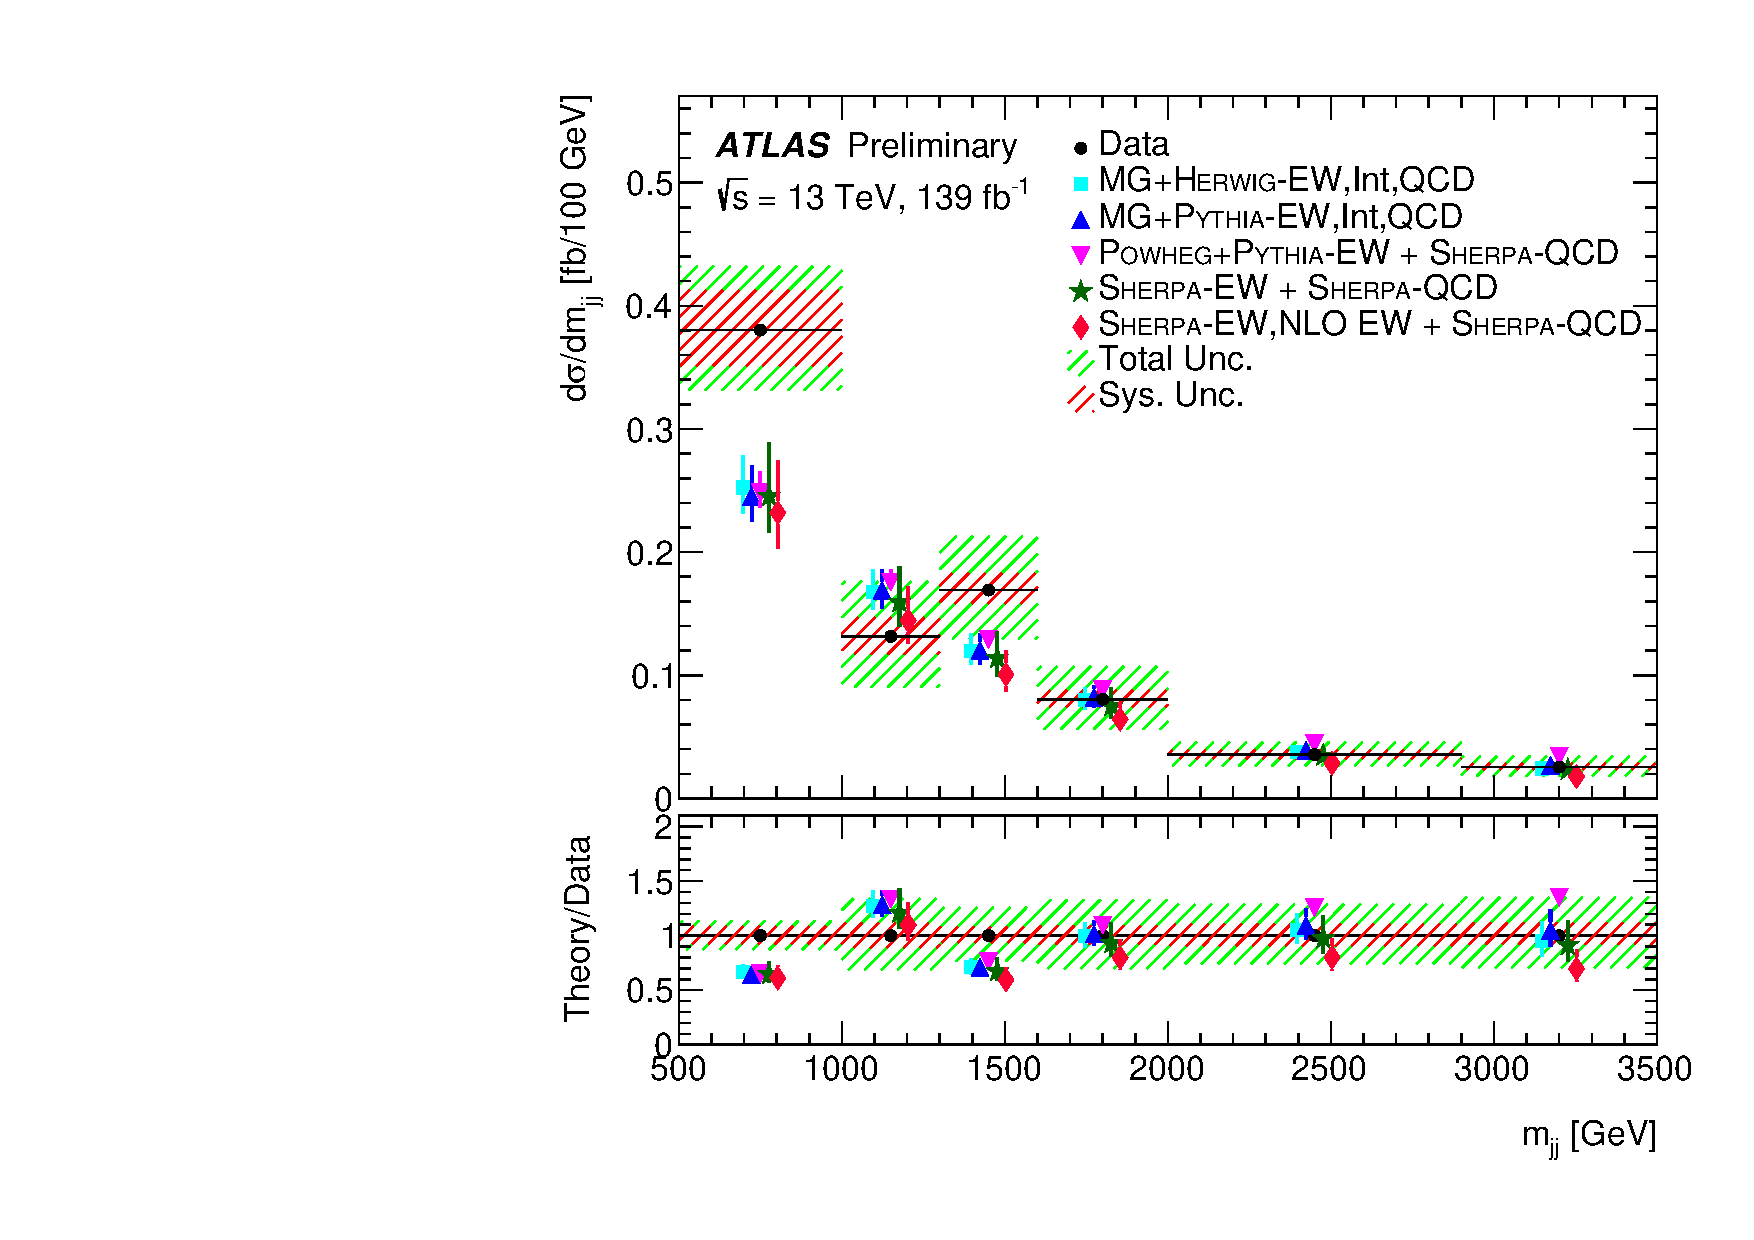
\includegraphics[width=0.49\textwidth]{figures/fig_06c.pdf}}
           \centering
       \end{minipage}
       \caption{Unfolded differential cross-sections of inclusive $W^\pm W^\pm jj$ production with $m_{ll}$ and $m_{jj}$.\protect\cite{ssww}}
\end{figure}\noindent
One and two-dimensional limits are set on Wilson coefficients corresponding to dimension-8 (dim-8) EFT operators. Dim-8 is the first time operators appear that only affect the quartic interactions. Since dim $>$ 4 operators can lead to scattering amplitudes that violate unitarity, the constraints are derived at $m_{WW}$ \footnote{An observable is chosen that quantifies the flow of energy through the $W^\pm W^\pm$ vertex.} cut-off energies which represent the un-unitarised and unitarised limits. The  cut-off values for the unitarised limits are given by the intersection of the unitary bounds derived from theory, and the observed 95\% confidence limits on $\frac{f}{\Lambda^4}$ (the Wilson coefficient divided by the cut-off energy). This cut-off represents the largest energy that flows through the $W^\pm W^\pm$ vertex that doesn't violate unitarity. In this analysis, the differential measurement of $m_{\mathrm{T}}$ is also used to set limits on the production of $H^{\pm\pm}$ decaying to $W^\pm W^\pm$, within the GM model. A $2.5\sigma$ global excess is observed consistent with a $H^{\pm\pm}$ of invariant mass $m(H^{\pm\pm})\approx450$ GeV.
% Include figure for mH here??

\section{Measurement of inclusive $ZZ(\rightarrow 4l)jj$ production}
Differential cross-section measurements of the inclusive production of $ZZ$ both decaying leptonically in association with jets ($ZZ(\rightarrow4l)jj$) is made using the ATLAS detector. The differential measurements are used to constrain aQGCs and anomalous Trilinear Gauge Couplings (aTGCs). \cite{zz4l}
$ZZ(\rightarrow 4l)jj$ is sensitive to quartic EW interactions through VBS. A signal region is defined by selecting for two same-flavour opposite-sign lepton pairs and two jets. In addition, events are selected for a VBS event topology (large dijet invariant mass, dijet rapidity gap, dijet \pt, and central 4-lepton system). As in section \ref{sec:ssww}, a binned log-likelihood fit is used to derive unitarised and un-unitarised limits. Limits are set on Wilson coefficients corresponding to dimension-8 and dimension-6 operators, where the parity-odd signed angular observables allow for tighter constraints on the Wilson coefficients of dimension-6 parity-odd operators.
%Can put differential cross-sections and/or constraints here

\section{Measurement of $Z(\rightarrow ll)\gamma\gamma$}
Quartic EW interactions can also be probed through triboson measurements. The triboson production of $Z(\rightarrow ll)\gamma\gamma$ is sensitive to potential BSM physics through an anomalous quartic interaction between neutral EW gauge bosons. %Insert feynman diagram here
Integrated fiducial cross-sections as well as differential cross-sections of $Z(\rightarrow ll)\gamma\gamma$ with photons originating purely from Initial State Radiation (ISR) are measured \cite{zyy}. The event selection criteria that facilitates this is given by the requirement $$m_{ll}+\mathrm{min}(m_{ll\gamma_1},m_{ll\gamma_2})>2m_Z,$$ where $m_{ll\gamma_1}$ and $m_{ll\gamma_2}$ refer to the invariant mass of the combined dilepton-photon system for leading or sub-leading photons, respectively, and $m_{Z}$ refers to the invariant mass of the $Z$ boson, i.e. approximately $91$ GeV. Previous measurements of $Z(\rightarrow ll)\gamma\gamma$ have been made by ATLAS at 8TeV \cite{zyy_atlas}, and CMS at 13TeV \cite{zyy_cms}, but without any FSR rejection. \\\\
The first differential cross-section measurements of the $Z(\rightarrow ll)\gamma\gamma$ are derived as a function of five observables ($E_{\mathrm{T},\gamma}$, $p_{\mathrm{T},ll}$, $p_{\mathrm{T},ll\gamma\gamma}$, $m_{\gamma\gamma}$, and $m_{\gamma\gamma ll}$). These are the transverse energy of the photon, dilepton transverse momentum, dilepton-diphoton transverse momentum, diphoton invariant mass, and dilepton-diphoton invariant mass. The $m_{\gamma\gamma}$ distribution is important in the context of diphoton resonance searches in $ll\gamma\gamma$ channels. The differential cross-section measurements are used to put constraints on dim-8 aQGC.
% Insert differential cross-sections here.

\section{Observation of $W\gamma\gamma$ production}
The first observation of triboson $W\gamma\gamma$ production at the LHC is made using the ATLAS detector \cite{wyy}. The fiducial cross-section of $W\gamma\gamma$ is also measured. $W(l\nu)\gamma\gamma$ is a challenging final state due to large non-prompt backgrounds, where objects are misreconstructed at detector level. The largest background is from hadronic fake photons, followed by the misreconstruction of electrons to photons, and hadronic fake leptons. The dominant uncertainties on the fiducial cross-section measurement come from the non-prompt background estimates. An observation is made at $5.6\sigma$, and a fiducial cross-section of $\sigma_{\mathrm{fid}}=12.2^{+2.1}_{-2.0}$ fb is measured.

\section{Observation of $WZ\gamma$ production}
The first observation and fiducial cross-section measurement of triboson $WZ\gamma$ at the LHC is made using the ATLAS detector \cite{wzy}. Previous measurements have observed combined VVV production \cite{vvv} by CMS, WWW production by ATLAS \cite{www}, and combined $WW\gamma$ and $WZ\gamma$ production by ATLAS \cite{wwywzy_atlas} and CMS \cite{wwywzy_cms}.\\
The measurement is performed in the fully leptonic final states in an FSR suppressed, ISR enhanced phasespace. This is facilitated by the dilepton invariant mass requirement $m_{ll}>81$ GeV. The largest backgrounds originate from $ZZ\gamma$ production, and $ZZ(e\rightarrow\gamma)$ production where one of the electrons from the leptonic Z decay is misreconstructed as a photon. Dedicated control regions are defined to constrain these two backgrounds. $WZ\gamma$ production is observed at $6.3\sigma$, and a fiducial cross-section measurement of $\sigma_{\mathrm{fid}}=2.01\pm0.30(\mathrm{stat.})\pm0.16(\mathrm{syst.})$ fb is made.
%Need conclusion and figures
\section{Conclusion}
It has been a very productive year for Standard Model EW triboson and VBS analyses. A number of new observations have been made of processes with cross-sections of the order of fb, where these processes often have large challenging backgrounds such as those from the irreducible strong production mode or from misreconstructed objects. New differential cross-section measurements of very rare EW processes in VBS or ISR enriched regions of phasespace have been made and form part of an increasingly large body of data which can be used to put state-of-the-art constraints on aQGCs. 
%\section*{Acknowledgments}
%
%This is where one places acknowledgments for funding bodies etc.
%Note that there are no section numbers for the Acknowledgments, Appendix
%or References.
%
\section*{References}

\begin{thebibliography}{99}
\bibitem{atlas} ATLAS Collaboration, 2008 JINST 3 S08003

\bibitem{osww} ATLAS Collaboration, ATLAS-CONF-2023-039, \url{http://cds.cern.ch/record/2865482}

\bibitem{ssww} ATLAS Collaboration, ATLAS-CONF-2023-023, \url{http://cds.cern.ch/record/2859330}

\bibitem{zz4l} ATLAS Collaboration, ATLAS-CONF-2023-024, \url{http://cds.cern.ch/record/2859349}

\bibitem{zyy} ATLAS Collaboration, EPJC 83 (2023) 539

\bibitem{zyy_atlas} ATLAS Collaboration, PRD 93, 112002

\bibitem{zyy_cms} CMS Collaboration, JHEP 10 174 (2021)

\bibitem{wyy} ATLAS Collaboration, ATLAS-CONF-2023-005, \url{http://cds.cern.ch/record/2853334}

\bibitem{wzy} ATLAS Collaboration, CERN-EP-2023-095, \url{http://cds.cern.ch/record/2860061}

\bibitem{vvv} CMS Collaboration, PRL 125, 151802 (2020)

\bibitem{www} ATLAS Collaboration, PRL 129, 061803 (2022)

\bibitem{wwywzy_atlas} ATLAS Collaboration, EPJC 77, 646 (2017)

\bibitem{wwywzy_cms} CMS Collaboration, PRD 90, 032008 (2014)

\end{thebibliography}

\end{document}

%%%%%%%%%%%%%%%%%%%%%%
% End of vietnam.tex %
%%%%%%%%%%%%%%%%%%%%%%
